\documentclass{article}

% Language setting
% Replace `english' with e.g. `spanish' to change the document language
\usepackage[english]{babel}

% Set page size and margins
% Replace `letterpaper' with`a4paper' for UK/EU standard size
\usepackage[letterpaper,top=2cm,bottom=2cm,left=3cm,right=3cm,marginparwidth=1.75cm]{geometry}


% Useful packages
\usepackage{amsmath}
\usepackage{graphicx}
\usepackage[colorlinks=true, allcolors=blue]{hyperref}

\title{Investigating Rust's Anonymous Symbols for Embedded Contexts}
\author{Gabe Barney}

\begin{document}
\maketitle

\section{The concept of embedded data and why it's important}

Embedded data is considered the disk space that is not necessarily allocated by the application, but rather the constructs of the compiler and language that increase the size of the binary. Currently, we detect embedded data by parsing for the space between different symbols which tells us how much padding there is, as well as the space that is used by constant strings.


\section{What I've looked at}

\subsection{Manually attributing symbols to functions on ARM}

\begin{figure}[h]
\centering
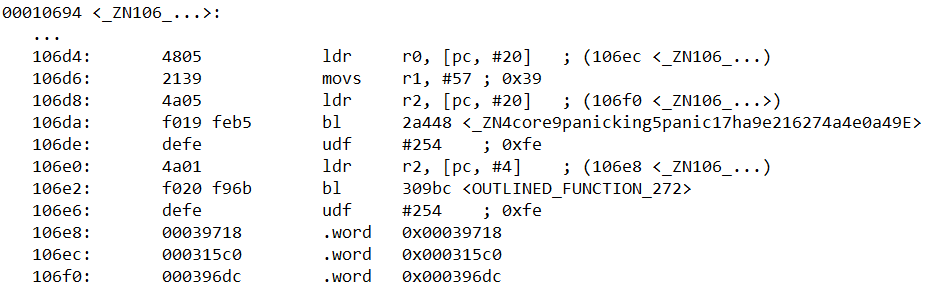
\includegraphics[width=.75\textwidth]{word_img.png}
\caption{\label{fig:word} An example of ldr instructions and ARM words}
\end{figure}
\begin{figure}[h]
\centering
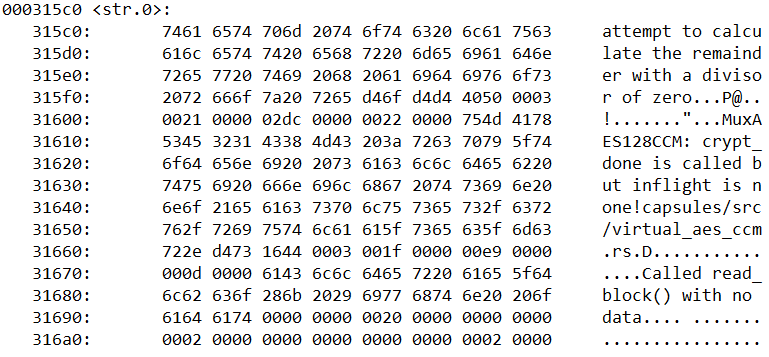
\includegraphics[width=.7\textwidth]{str0_img.png}
\caption{\label{fig:str0}An example symbol in ARM's literal pool}
\end{figure}

In ARM, there are '.word' directives which are a level of indirection that makes parsing symbols directly through pure string manipulation very difficult because of address alignment. Compounding upon this, because words are an arbitrary directive, we can't always tell what the meaning for each of the words for functions mean. This is because there are sometimes words that are generated to be used for padding in order to align the literals in the literal pools. We can't understand these automatically generated words without looking into each individual case. Another issue is that when we find the location of a word, often times we don't know the length, due to the difficulty of trying to manually parse registers. With some functions, such as basic panics such as in \autoref{fig:word}, it is easy to understand the length of the literal that's being referred to, but we find that the coverage of this byte-wise isn't nearly as significant as we would hope.

Approximately ~52\% of the imix board embedded data is panic-related, this is deduced by removing the panic handler and comparing binary sizes. By parsing the length of strings used in panics by detecting the string length registers, which in \autoref{fig:word}'s case is r1, there is a surprisingly low ~8\% of this panic-related data that is attributed with this method. And this is the majority case of panic data that we can detect manually. It is also by far the simplest.

The main issue that occurs here seems to be rooted in ARM's literal pooling. Parsing strings, like in \autoref{fig:str0}, is difficult when they're in such large collections with unrelated strings immediately surrounding them. We can easily attribute the first string in Figure 2 from Figure 1's assembly through string manipulation, but what about cases that aren't as explicit and straightforward as panics? Additionally, ARM seems to mix in unreferenced embedded strings with referenced ones, which greatly adds to the complexity when we were looking at the imix binary.

It's not a simple task to detect embedded data in ARM, you would expect that looking at the symbol table would easily give you the size of all the embedded string symbols, even if they're clumped together with unrelated strings. But it turns out that the symbol sizes in the symbol table are the size of only the first string in that symbol. This means that any string past the first string is not detected in the size of that symbol, and that you could only really detect the true overall size of a symbol by looking at the difference in the addresses from one symbol to its neighbor.

With ARM, there is limited 4KB offset for the LDR instruction, which can make it understandable that there are some oddities in ARM's literal pool. This gives some inspiration to changes in platform to RISC-V that can be read in Section 2.4.

\subsection{llvm-dwarfdump and pyelftools}

Quickly realizing that manually parsing lengths of these anonymous symbols is too difficult, especially for such low coverage. Trying to leverage the ELF and DWARF tooling available became attractive, as it would be far more generalized. This would be beneficial because we could get more coverage of the panics, as well as attribute embedded data to more functions beyond just panics.

\begin{figure}[h]
\centering
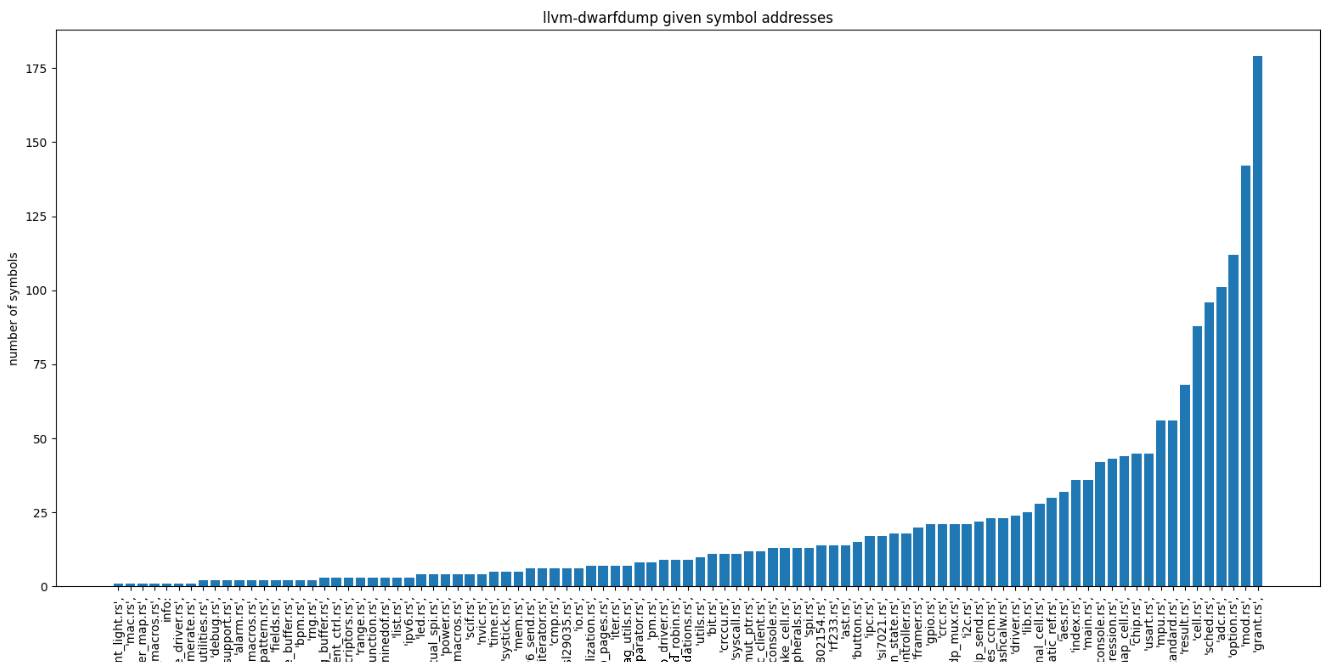
\includegraphics[width=\textwidth]{dwarfdump_img.png}
\caption{\label{fig:dwarfdump}This plot shows how often these tools attribute symbols to files}
\end{figure}

I believe that pyelftools\footnote{\url{https://github.com/eliben/pyelftools}} could be particularly useful for attributing symbols to functions, but its surface value seems to be equivalent of llvm-dwarfdump. LLVM's dwarfdump is simply faster, so I resorted to using it after a brief testing period.

From \autoref{fig:dwarfdump}, we can see that the tool doesn't seem to have an inappropriate attribution scheme, and can attribute embedded data to files and line numbers. But the different DWARF outputs from similar embedded data made it obscure to establish further findings, particularly the functions in which they occur. The tools output the line and column numbers of where the symbols should be, but it is still completely uncertain how or where the embedded data comes into play. These locations that are received don't quite output interesting code, and make it seem that this doesn't quite achieve what is wanted. There is potential promise, but it seems to be best left alone for now. Those with extensive DWARF experience could probably figure out more.

\subsection{Determining the influence of LLVM's Link Time Optimization}

Discussion led to investigating how LTO affects the organization of the binary in ARM. It caused a minor increase in number of symbols, but made no clear improvement in the ability to easily parse and attribute strings to functions, as they were still heavily clumped together with unrelated strings. The importance in this is that this further cements the conclusion that this is most likely an issue with ARM.

\subsection{RISC-V analysis}

The lack of meaningful information gained from turning off LTO on ARM prompted looking at a RISC-V board. Coming into this without knowing any differences between ARM and RISC-V, it was natural to check if LTO has any influence on RISC-V, then attempting to see how easily symbols can be attributed to functions, like in Section 2.1.

Having LTO off has 779 symbols related to embedded data while having LTO on has 675 symbols related to embedded data. This makes intuitive sense.

In RISC-V, there is a new symbol type. It's titled L\_\_unnamed, yet its functionality seems identical to Lanon symbols. Yet, turning LTO on causes there to be more Lanon than unnamed, and turning LTO off causes there to be more unnamed than Lanon. It seems there's no functional difference between these two different symbol types, but their change in distribution with LTO turned on/off is interesting. Additionally, there seems to be a range, increasing from 170, in the \_\_unnamed\_ symbol naming scheme that corresponds to them being unreferenced.

\begin{figure}[h]
\centering
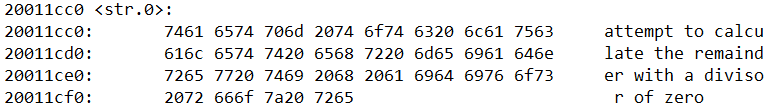
\includegraphics[width=.8\textwidth]{riscv_str0_img.png}
\caption{\label{fig:riscv_str0}An example symbol in RISC-V's literal pool}
\end{figure}

\begin{figure}[h]
\centering
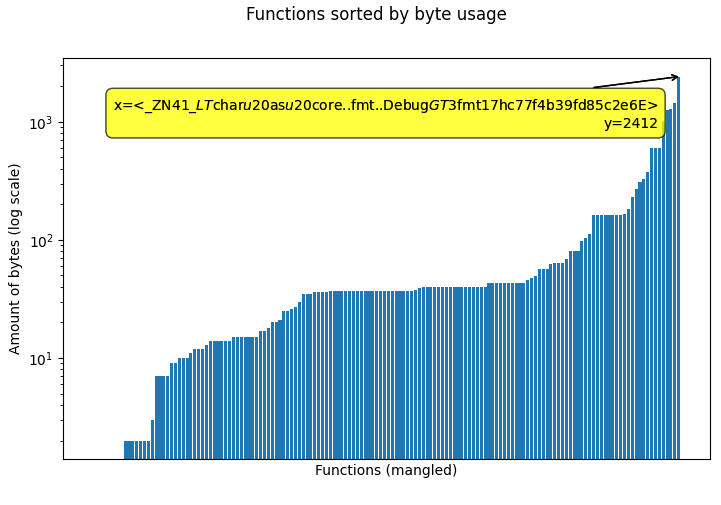
\includegraphics[width=.8\textwidth]{byte_usage_plot.png}
\caption{\label{fig:byte_usage}A plot showing the embedded string byte contribution per function}
\end{figure}

It's reasonable to believe that the limitation on LDR offsets, is a potential reason for the literal pool issues, and is therefore the reason why ARM is so hard to parse. There is no behavior alike this limitation on LDRs in RISC-V. When looking at symbols in RISC-V that were clumped together in ARM, they are completely isolated to themselves.

This property of RISC-V, along with the removal of the words from ARM, make it very easy to parse through the assembly and attribute the symbols to functions. Making attributions and code size contributions for functions simple. From the limited information visible in  \autoref{fig:byte_usage}, I've completed a mapping of functions to their embedded string byte usages. This also means t hat it's possible to know the mapping of all the symbols to their functions they're used in.

Given the long names of functions as well as the difficulty in representing the y-axis, if you want to know the details of this plot, as well as other related plots, you'll need to hover over the bar by graphs using the script or the notebook. \footnote{\url{https://github.com/barneyga/tock-embedded-data}}

\subsection{Next steps}
\begin{enumerate}
    \item Embedded data detection doesn't work the same for RISC-V boards as it does with ARM board. This makes it hard to comprehend the coverage we get from mapping the symbols to their functions.
    
    \item Following from this, being able to isolate certain functions and determine their coverage and individual attributes, currently I can only think of compiling without the panic handler, as done before, but I'm unsure as to how other features could be isolated.
    
    \item Expanding the current print\_tock\_memory script with a flag that prints information about the embedded data organized by their parent functions.
\end{enumerate}
\end{document}